\documentclass[12pt,a4paper]{report} % 'report' es ideal para tesis
\usepackage[utf8]{inputenc}   % para acentos
\usepackage{hyperref}         % para enlaces
\usepackage{graphicx}		  % para imágenes
\usepackage{float}



\begin{document}
	
	\title{NutriPlan}
	\author{Aissa Rouk El Masoudi}
	\maketitle
	
	\section*{Resumen}
	OMS cita que en 2022 el 43\% de los adultos en el mundo tenía sobrepeso, y el 16\% padecía obesidad, lo que equivale a unos 890 millones de adultos obesos\cite{OMSObesidadySobrepeso}. Desde 1990, el número de personas con obesidad se han más que duplicado entre los adultos y se han cuadruplicado entre los adolescentes\cite{ONUAAComercioAlimentosyObesidad}.
	\\Esta situación afecta a personas de todas las edades, regiones y tiene graves consecuencias para la salud, economía y los sistemas sanitarios, hace cada vez más urgente fomentar hábitos alimentarios saludables y estrategias que promuevan una alimentación consciente, eficiente y sostenible.
	%
	\\\\De este contexto surge NutriPlan, una aplicación de Meal Planning y gestión de recetas cuyo objetivo es fomentar un estilo de vida saludable, económico y sostenible, reduciendo el desperdicio de alimentos. 
	Esta idea surgió en mi experiencia como estudiante Erasmus, dónde descubrí que al realizar la lista de la compra manualmente y verificar cuáles ingredientes tenía, se ahorraba más dinero en la compra, desperdiciaba menos comida y lo más importante, comía sano.

	
	
	\section*{Motivación}
	Siempre quise crear algo relacionado con mis dos vocaciones, ayudar a las personas y la programación, cada vez que tengo un momento libre intento utilizarlo para pensar cómo hacer el mundo un sitio mejor, qué ideas de aplicaciones podrían aportar algo a las necesidades de la sociedad, esto me llevó a crear varias aplicaciones desde crear una aplicación de escritura reflexiva para mejora personal, hasta la creación de un software administrador de tareas.
	\\
	Esta idea de proyecto surgió cuando estaba en un programa de movilidad estudiantil, después de varios meses realizando la compra e intentando reducir su gasto sin que baje la calidad de mi dieta, noté al principio que cuando realizaba una lista de la compra, gastaba mucho menos de lo que debía, porque no compraba cosas innecesarias o duplicadas. Al cabo de otro tiempo, descubrí que si realizaba mi plan dietético de manera específica antes de realizar la compra semanal, este gasto era mucho menor porque en la lista añadía las cantidades de cada ingrediente que necesitaba, esto no solo redujo mis compras innecesarias, sino que me motivaba a comprar las cantidades exactas necesarias de cada producto o ingrediente, reduciendo el coste de mi compra semanal. 
	\\
	Además de este beneficio económico, percibí que la realización de esta práctica me impulsaba a respetar las cantidades planificadas en mi dieta, haciendo que, esta no solo se volviera más saludable, sino también más variada.
	La Librería Nacional de Medicina Estadounidense realizó un estudio dónde se concluyó que \textit{“la planificación dietética está asociada a una dieta más saludable y una menor prevalencia de obesidad”}\cite{NLMMealPlanningBenefits}, y que \textit{“la práctica de esta podría ser potencialmente relevante para la prevención de la obesidad”}\cite{NLMMealPlanningBenefits}. 
	\\
	Una publicación de la Comisión Europea afirma que los hogares generan más de la mitad del desperdicio alimentario existente y que una de sus causas es la insuficiente planificación de las compras y de las comidas, lo que no solo perjudica la economía familiar, sino que también tiene un impacto ambiental significativo.
	\\
	Todo esto me llevó a crear NutriPlan, una aplicación que satisface todas estas necesidades. Un software que ayuda a los usuarios mediante la creación de una lista de la compra con las recetas ya registradas por el usuario, lleva un seguimiento de su despensa recordando que ingredientes aún tiene disponibles, y calculando cuándo cada ingrediente que se acaba.
	
	\section*{Objetivos}
	
	El objetivo de este proyecto es la creación de una aplicación móvil que facilite la planificación dietética, haciéndola más sencilla y eficiente promoviendo todos los beneficios discutidos anteriormente en la motivación; lleve un seguimiento de la despensa del usuario y modifique esta cada vez que se realice la compra, planificación de la dieta semanal mediante la adición o eliminación de ingredientes en la despensa.
	\\
	\\
	El resultado será una aplicación con las siguientes funcionalidades:
	
	
	\begin{itemize}
		\item Gestión de recetas
		\begin{itemize}
			\item Adición de una nueva receta mediante la introducción del nombre, enlace, tiempo de preparación y la cantidad de porciones de la receta; la adición de los ingredientes correspondientes a la receta.
			\item Eliminación o edición de una receta ya existente.
		\end{itemize}
		
		\item Gestión de ingredientes
		\begin{itemize}
			\item Adición de nuevos ingredientes a una receta con sus cantidades.
			\item Posibilidad de buscar (mediante un motor de búsqueda) ingredientes nuevos para añadirlos a una receta que se esté creando.
		\end{itemize}
		
		\item Gestión de dieta semanal
		\begin{itemize}
			\item El usuario podrá asignar una o varias recetas para cada comida del día (desayuno, comida, cena), esta asignación es modificable.
		\end{itemize}
		
		\item Gestión de la lista de la compra
		\begin{itemize}
			\item El programa será el encargado de la creación de una lista de la compra. Esto se realizará sumando las cantidades de los ingredientes similares de todas las recetas y restando a esta suma las cantidades que haya en la despensa.
		\end{itemize}
	\end{itemize}


	\section*{Metodología del proyecto}
	
	
		El desarrollo de esta aplicación se ha estructurado en cinco fases, cada una con finalidades específicas para garantizar la evolución coherente y eficiente de este proyecto.
	
	\begin{enumerate}
	
		\item Revisión bibliográfica y justificación
		
		En esta fase se llevó a cabo una exhaustiva investigación de estudios y publicaciones científicas sobre la planificación dietética y su impacto en la salud, el ahorro económico y el desperdicio de alimentos. Esta investigación nos proporciona una base sólida para justificar la necesidad y relevancia de esta aplicación para nuestra sociedad.
		
	
		
		\item Diseño de la solución
		
		Se definieron las funcionalidades de la aplicación, como la creación de recetas, la planificación de menús, el seguimiento de la despensa y la generación de la lista de compra. Además, se seleccionaron las tecnologías y herramientas que se utilizarán para el desarrollo cómo Firebase(backend), React Native(frontend), Android Studio(teseo)
		
	
		\item Desarrollo técnico
		
		En esta etapa, se procedió a la creación y implementación de acuerdo con las funcionalidades y tecnologías definidas y seleccionadas anteriormente. Se desarrollaron los componentes como la interfaz de usuario, las funcionalidades, estructura de datos su gestión y almacenamiento. Se utilizó el control de versiones para mantener un desarrollo ordenado y fluido.
		
		
		\item Pruebas y finalización
		
		Se realizaron pruebas para verificar el correcto funcionamiento de la aplicación creada. El software fue usado por un período para identificar errores o posibles mejoras y estos fueron identificados y resueltos.
		
	\end{enumerate}

	
	\section*{Estado del arte}
	
	
	\subsubsection*{La planificación dietética o Meal prepping}
	
	Hoy en día es difícil tener un estilo de vida saludable dada la falta de tiempo que causan las responsabilidades como el trabajo, familia, sueño, etc; varios datos muestran que los jóvenes consumen mucha menos fruta y verdura de la cantidad recomendada diaria, y que estos consumen mucho más comida basura de la que se recomienda \cite{NLMDifficultyEatingHealthy}.
	\\
	Otro análisis indica que la mayor barrera que impide a las personas de seguir una dieta saludable es la falta de tiempo, el no querer abandonar alimentos favoritos y los elevados precios de las comidas sanas \cite{NLMDifficultyEatingHealthy}. A mucha gente le cuesta mantener ese balance entre trabajar y tener una vida sana y he de ahí donde surge la planificación de dietas o meal planning, una práctica que consiste en planificar las comidas de un periodo futuro determinado(generalmente una semana). La mayor parte de las personas planifican tres comidas por día para los días laborales(de lunes a viernes), pero esta práctica es completamente personalizable.\cite{HowToMealPrep}.
	\\
	\\
	
	El método de uso de esta práctica puede variar dependiendo de la persona, pero la metodología más común es la siguiente.
	
	%
	% Pasos para crear una lista de la compra
	%
	\begin{enumerate}
		\item Se elabora una tabla en la que se escriben todos los días de la semana en las columnas y los tipos de comida (desayuno, comida, cena, y en su caso merienda o aperitivo) en las filas  (Figura~\ref{fig:Plantillamealplan}). En cada celda se anotan las recetas o alimentos que se consumirán en el día y la comida correspondiente. A pesar de que este proceso se puede realizar en papel, resulta preferible hacerlo en un ordenador ya que facilita la edición y corrección de posibles errores. La tabla resultante será similar a la de la Figura~\ref{fig:Plantillamealplanrellenada}.
		
		\begin{figure}[H]
			\centering
			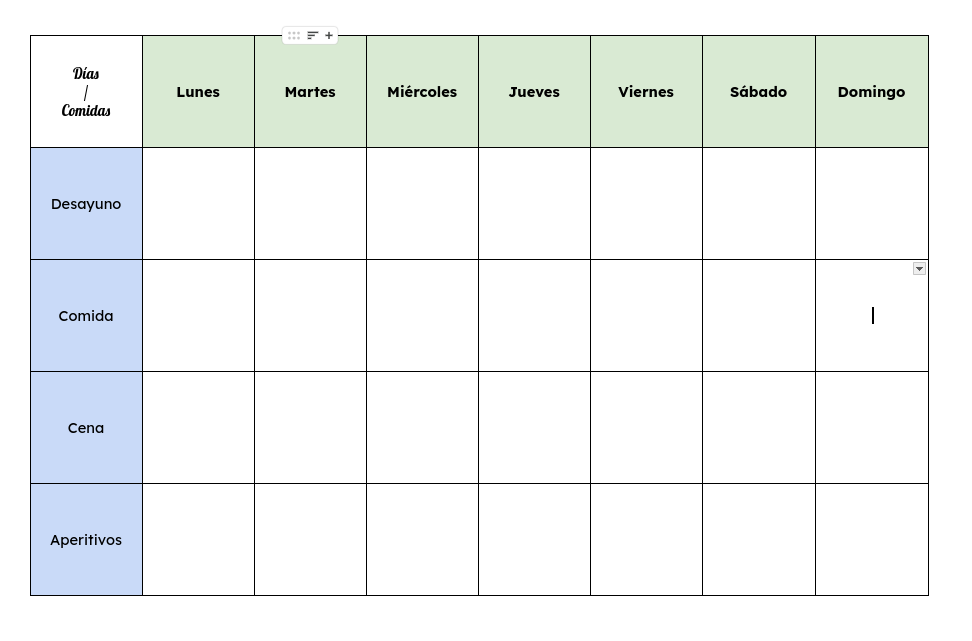
\includegraphics[width=1\textwidth]{./PlantillaTablaMealPlanning.png}
			\caption{Plantilla planificación de comidas}
			\label{fig:Plantillamealplan}
		\end{figure}	
	
		\begin{figure}[H]
			\centering
			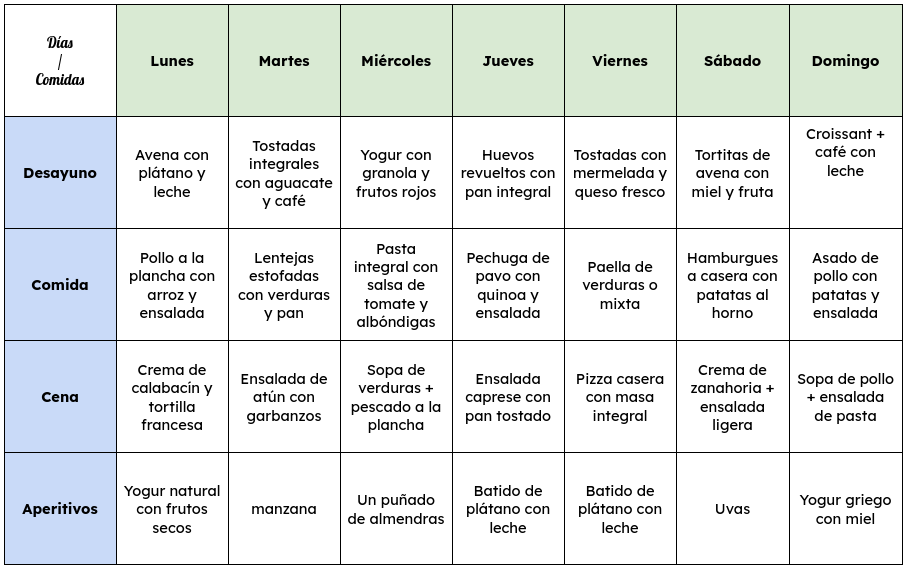
\includegraphics[width=1\textwidth]{./PlantillaMealPlanningRellenada.png}
			\caption{Plantilla planificación de comidas}
			\label{fig:Plantillamealplanrellenada}
		\end{figure}	
		
		\item Una vez completada la tabla con las recetas de la semana, se procede a listar los ingredientes necesarios para su preparación, incluyendo las cantidades específicas de cada uno (ver Tablas ~\ref{fig:TablaDeIngredientes} y ~\ref{fig:TablaCombinada}).
		
		\begin{table}[H]
			\centering
			\caption{Ejemplo de recetas con ingredientes comunes}
			
			\begin{tabular}{|p{3.5cm}|p{7cm}|p{3cm}|}
				\hline
				\textbf{Receta} & \textbf{Ingredientes} & \textbf{Cantidad (para 2 personas)} \\ \hline
				
				Pollo a la plancha con arroz y ensalada 
				& Pechugas de pollo, arroz, lechuga, tomate, aceite de oliva, sal, pimienta, limón 
				& Pollo 300 g; Arroz 120 g; Lechuga 100 g; Tomate 100 g; Aceite 10 ml \\ \hline
				
				Asado de pollo con patatas y verduras 
				& Pollo, patatas, zanahoria, cebolla, aceite de oliva, sal, pimienta, romero 
				& Pollo 500 g; Patatas 400 g; Zanahoria 200 g; Cebolla 100 g; Aceite 20 ml \\ \hline
			\end{tabular}
			\label{fig:TablaDeIngredientes}
		\end{table}
		
		\begin{table}[H]
			\centering
			\caption{Lista de la compra combinada (optimizada)}

			\begin{tabular}{|p{5cm}|p{3cm}|}
				\hline
				\textbf{Ingredientes} & \textbf{Cantidad total} \\ \hline
				Pollo & 800 g \\ \hline
				Arroz & 120 g \\ \hline
				Lechuga & 100 g \\ \hline
				Tomate & 100 g \\ \hline
				Patatas & 400 g \\ \hline
				Zanahoria & 200 g \\ \hline
				Cebolla & 100 g \\ \hline
				Aceite de oliva & 30 ml \\ \hline
				Condimentos (sal, pimienta, romero, limón) & Al gusto \\ \hline
			\end{tabular}
			\label{fig:TablaCombinada}
		\end{table}
		
		
		\item Al obtener la lista de ingredientes necesarios para preparar las recetas planificadas, se revisan los productos disponibles en el hogar(en el caso de un usuario común, el hogar). Esto permite la identificación de ingredientes que ya se poseen, haciendo que se puedan eliminar de la lista y ajustar la cantidad de los que se tengan parcialmente, evitando compras innecesarias y reduciendo el desperdicio alimentario. En nuestro ejemplo se supondrá que la despensa tiene 500 gramos de pollo y 100 de arroz(Tabla~\ref{fig:TablaCalculoIngr}), dando a la tabla de ingredientes final(Tabla~\ref{fig:TablaIngrFinal}))
		
		% Tabla de ingredientes a comprar y en despensa
		
		\begin{table}[H]
			\label{fig:TablaCalculoIngr}
			\centering
			\caption{Proceso de cálculo de ingredientes según la despensa}
			\begin{tabular}{|p{3cm}|p{3cm}|p{3cm}|p{3cm}|}
				\hline
				\textbf{Ingredientes} & \textbf{Necesario} & \textbf{En despensa} & \textbf{A comprar} \\ \hline
				Pollo & 800 g & 500 g & 300 g \\ \hline
				Arroz & 120 g & 100 g & 20 g \\ \hline
				Lechuga & 100 g & 0 & 100 g \\ \hline
				Tomate & 100 g & 0 & 100 g \\ \hline
				Patatas & 400 g & 0 & 400 g \\ \hline
				Zanahoria & 200 g & 0 & 200 g \\ \hline
				Cebolla & 100 g & 0 & 100 g \\ \hline
				Aceite de oliva & 30 ml & 0 & 30 ml \\ \hline
				Condimentos & Al gusto & 0 & Al gusto \\ \hline
			\end{tabular}
		\end{table}
		
		% Tabla de ingredientes finales
		
		\begin{table}[H]
			\centering			
			\label{fig:TablaIngrFinal}
			\caption{Lista de la compra final optimizada}
			\begin{tabular}{|p{5cm}|p{3cm}|}
				\hline
				\textbf{Ingredientes} & \textbf{Cantidad a comprar} \\ \hline
				Pollo & 300 g \\ \hline
				Arroz & 20 g \\ \hline
				Lechuga & 100 g \\ \hline
				Tomate & 100 g \\ \hline
				Patatas & 400 g \\ \hline
				Zanahoria & 200 g \\ \hline
				Cebolla & 100 g \\ \hline
				Aceite de oliva & 30 ml \\ \hline
				Condimentos (sal, pimienta, romero, limón) & Al gusto \\ \hline
			\end{tabular}
		\end{table}
		
		
		
		\item Ahora que se ha obtenido la lista definitiva, es recomendable revisar la lista para ver si falta o se ha duplicado algún ingrediente, este paso no es necesario, pero ayuda a prevenir fallos. Después de esto faltaría solo realizar la compra.
	\end{enumerate}


	En los últimos años la planificación dietética ha ganado popularidad gracias a diversos factores sociales y culturales. De entre ellos destacan el auge de las redes sociales y la creciente influencia del culturismo y el deporte en la vida cotidiana. Plataformas como Instagram, YouTube o TikTok han facilitado el acceso a información sobre estos tópicos, motivando a muchos a estructurar sus dietas de forma más consciente y personalizada. Esta tendencia se observa también en el ámbito deportivo, como por ejemplo en el culturismo, donde el \textit{meal planning} es una práctica habitual y está estrechamente ligada a la preparación física. Varios estudios recientes muestran que los practicantes del culturismo adoptan esta práctica como parte fundamental de su entrenamiento, y que su fuente de información principal son las redes sociales y la comunidad digital \cite{helms2019,masoga2021,benjamins2021}.
	\\	
	Este fenómeno no solo se refleja en ámbitos deportivos como el culturismo, sino también en la población general. Una investigación francesa descubrió que el 57,4\% de los habitantes planifican sus comidas al menos de manera ocasional, lo que evidencia un interés extendido en esta práctica como parte de la vida diaria \cite{ducrot2017}. De manera similar, en los Estados Unidos se estima que alrededor del 37\% organizan sus comidas con uno o dos días de antelación, lo que muestra el aumento del uso de la programación de menús fuera del ámbito deportivo \cite{fmi2015}. Esta convergencia entre el impacto social de las plataformas digitales, las prácticas del culturismo y la creciente adopción de \textit{meal planning} en la población aporta una razón y contexto sólidos para el desarrollo de herramientas digitales como \textit{NutriPlan}, cuyo objetivo es facilitar la organización alimentaria de manera sencilla, eficiente y accesible.
	\\\\
	El mercado de aplicaciones de planificación dietética está en constante expansión. Durante 2024 su valor alcanzó los 2,21 millones de dólares y se proyecta que crecerá al valor de 5,53 millones en 2033 \cite{businessresearchinsights2024}. Esta expansión viene impulsada por las nuevas tendencias como la de integración de la inteligencia artificial para la personalización de menús, la incorporación de prácticas sostenibles y la creación de comunidades digitales en torno a la alimentación. Además, la pandemia Covid-19 aceleró esta adopción al fomentar la preparación de comidas en casa y la planificación de las compras. Si se añade a la perspectiva el informe a nivel global de McKinsey, donde se afirma que el 50\% de los consumidores prioriza una alimentación saludable y más del 70\% desea mejorar su dieta, se demuestra un gran interés en este tópico \cite{mckinsey2023}.
	\\\\
	Los beneficios que aporta la planificación dietética son los que generan el interés por este movimiento, caracterizada por la falta de tiempo para funciones básicas como el sueño, la práctica de deporte o la cocina. La organización de comidas no sólo asegura una ingesta calórica y nutricional adecuada, sino que también contribuye en diversos aspectos de la vida diaria.\\
	\textbf{Ahorro de tiempo.} Una de las principales dificultades para mantener hábitos alimenticios saludables es la falta de tiempo. Según análisis hechos por la Biblioteca Nacional de Medicina de EE. UU., esta práctica reduce las compras improvisadas durante la semana y el tiempo empleado en decidir qué cocinar cada día, mejorando la eficiencia y disminuyendo la improvisación.
	\\
	\textbf{Reducción del estrés.} El meal planning ayuda a disminuir la tensión y el estrés derivados de la indecisión diaria sobre qué comer. Muchas personas deciden qué cocinar o comer en momentos de fatiga o poca motivación, lo que les conduce a optar por opciones menos saludables. Disponer de un plan y de los ingredientes necesarios facilita la elección de comidas más equilibradas y reduce la carga mental asociada a esta tarea.
	\\
	\textbf{Mejora de la dieta.} Diversos estudios han demostrado que cocinar en casa con mayor frecuencia se asocia a un consumo menor de carbohidratos, azúcares y grasas \cite{johnshopkins2014}. Además, la planificación dietética incentiva a cumplir objetivos calóricos y nutricionales mediante la compra anticipada de ingredientes. La evidencia científica indica que esta práctica está relacionada con una mejor calidad de dieta y una menor prevalencia de obesidad, lo que la hace potencialmente relevante en estrategias de prevención \cite{ducrot2017}.
	\\
	\textbf{Ahorro económico.} El uso de una lista de la compra estructurada se asocia con una mayor calidad de la dieta y, al mismo tiempo, un gasto más eficiente, ya que evita la adquisición de productos innecesarios \cite{jneb2017}, haciendo que ésta práctica beneficie tanto a la salud como a la economía.
	\\
	\textbf{Reducción del desperdicio alimentario.} Más de 59 millones de toneladas de residuos alimentarios, con un valor estimado en 132 millones; son generados anualmente en la Unión Europea. Una de las principales causas identificadas es la falta de planificación en la compra de alimentos en los hogares \cite{europeancommission2020}. El \textit{meal planning} contribuye en la mitigación de este problema, al fomentar la compra de cantidades ajustadas a las necesidades reales.
	
	
	\subsubsection*{Aplicaciones móviles existentes de meal planning}
	El creciente interés en la planificación dietética ha impulsado el desarrollo de diversas aplicaciones móviles que buscan simplificar este proceso y adaptarlo a las necesidades del usuario. Algunas de las más conocidas son \textit{Mealime}, \textit{Yazio} e \textit{Instacart}.\\
	
	%Tabla comparativa de apps
	\begin{table}[H]
		\centering

		\begin{tabular}{|p{3cm}|p{5cm}|p{5cm}|}
			\hline
			\textbf{Aplicación} & \textbf{Funcionalidades principales} & \textbf{Limitaciones} \\ \hline
			
			\textbf{Mealime} & 
			- Creación de menús semanales personalizados. \newline
			- Generación automática de lista de la compra. \newline
			- Recetas adaptadas a preferencias básicas. & 
			- Personalización limitada (no permite modificar recetas de forma profunda). \newline
			- Algunas funciones solo disponibles en versión de pago. \\ \hline
			
			\textbf{Yazio} & 
			- Planificación de comidas integrada con conteo calórico. \newline
			- Seguimiento de macronutrientes y calorías. \newline
			- Integración con objetivos de salud y pérdida de peso. & 
			- Interfaz compleja para usuarios novatos. \newline
			- Funcionalidades avanzadas bloqueadas en versión premium. \\ \hline
			
			\textbf{Instacart} & 
			- Planificación de comidas vinculada al comercio electrónico. \newline
			- Compra directa de ingredientes desde recetas seleccionadas. & 
			- Dependencia de supermercados asociados. \newline
			- Menor enfoque en personalización dietética y salud. \\ \hline
			
			\textbf{NutriPlan (Propuesta)} & 
			- Creación de recetas personalizadas con control absoluto de ingredientes. \newline
			- Planificación semanal flexible (desayuno, comida, cena). \newline
			- Generación automática de lista de la compra optimizada. \newline
			- Gestión de la despensa con actualización automática. & 
			- En desarrollo, pendiente de validación con usuarios reales. \newline
			- Requiere uso inicial de tiempo para registrar recetas propias. \\ \hline

		\end{tabular}			
		\caption{Comparativa de aplicaciones de meal planning}
		\label{tab:comparativa_apps}
	\end{table}
	
	Como se observa en la Tabla~\ref{tab:comparativa_apps}, a pesar de que Mealime y Yazio ofrecen planificación básica y seguimiento nutricional, ambas dependen de versiones premium para acceder a sus funcionalidades completas. En el caso de Instacart, en cambio, está más orientada al comercio electrónico que a la salud. Frente a ello, NutriPlan aporta una mayor flexibilidad al permitir la creación de recetas personalizadas y gestionar la despensa, optimizando así la lista de la compra.
	\\
	
	\section*{Diseño de la solución}
	
	%\section*{Metodología de desarrollo}
	
	%El desarrollo de \textit{NutriPlan} se llevó a cabo de manera individual, siguiendo un enfoque híbrido que combina una planificación inicial con un proceso de trabajo iterativo e incremental. 
	
	%En una primera fase, se definió la estructura general de la aplicación, las funcionalidades principales y la organización de la información en la base de datos. Sin embargo, durante el desarrollo surgieron ajustes y nuevas ideas que fueron incorporadas de manera progresiva, lo que permitió refinar el producto de forma flexible.
	
	%El proceso de trabajo se organizó a través de la herramienta \textit{GitHub Projects}, utilizando un tablero dividido en tres columnas: \textit{pendiente}, \textit{en progreso} y \textit{finalizado}. Esta metodología, inspirada en el sistema Kanban, facilitó la gestión de tareas y la trazabilidad del avance, permitiendo mantener un control claro sobre el estado del proyecto.
	
	%Cada módulo de la aplicación (gestión de recetas, gestión de despensa, lista de la compra, etc.) se desarrolló de manera incremental, con pruebas continuas que permitieron identificar errores y añadir mejoras antes de avanzar a la siguiente etapa. Este ciclo iterativo de planificación, desarrollo, prueba y ajuste contribuyó a la calidad y robustez del producto final.
	
	
	
	\subsection*{Metodología de desarrollo}
	El desarrollo de la \textit{NutriPlan} se realizó de manera individual, siguiendo un enfoque hibrido que combina una planificación inicial con un proceso de trabajo iterativo e incremental.

	\subsection*{Arquitectura general de la aplicación}
	
	En la primera fase, se definieron las tecnologías usadas para el desarrollo de la aplicación, las funciones principales, la organización de la información en la base de datos y la estructura general de la aplicación.
	
	\subsubsection*{Tecnologías usadas para el desarrollo.}

	Se ha optado por el uso del framework \textit{React Native} para la implementación de las funcionalidades y el diseño, ya que permite generar aplicaciones multiplataforma (Android \& iOS) a partir de un código único en JavaScript, reduciendo tiempos y costes de desarrollo \cite{reactNative}, tiene una gran comunidad respaldada y mantenida por Meta, lo que asegura la abundancia y calidad de la documentación, soporte y librerías de terceros \cite{reactNativeComnty}; el rendimiento de esta es similar al de los programas nativos, obteniendo una experiencia de usuario fluida similar a apps desarrolladas en Java/Kotlin(Android) o Swift(iOS)\cite{reactNativeRnd}. Por otra parte la reducción que implica usar este código para diferentes plataformas permite ahorrar mucho tiempo y rendimiento, el 90\% del código está compartido entre iOS y Android. Otra de las razones de la elección de este framework es su carácter intuitivo, dado que está basado en \textit{JavaScript} y \textit{React} lo que lo hace más fácil a los programadores con expriencia web o en JavaScript a aprenderlo ya que la construcción de interfaces se realiza mediante componentes reutilizables \cite{reactnative2025}.
	\\
	En el caso de la base de datos se ha utilizado Firebase para su creación, esta es una plataforma de desarrollo de aplicaciones creada por Google que ofrece varios servicios en la nube, como la gestión de base de datos en tiempo real, autenticación de usuarios y \textit{hosting} \cite{firebase}, Haciendo que todas estas operaciones de autenticación y base de datos se ejecuten en la nube mejorando el rendimiento de la aplicación.
	\\
	Se optó por Github como plataforma de control de versiones debido a su versatilidad, compatibilidad con las demás plataformas y su integración directa con su sistema de control de cambios llamado Git. Este software no sólo te permite tener un historial de todos los cambios realizados en el código y restaurar versiones del código anteriores, sino que también proporciona Github Projects, una herramienta de organización de tareas \cite{github2025}.\\
	Además al ser la plataforma más utilizada a nivel mundial, cuenta con una amplia comunidad y gran cantidad de documentación.
	
	
	%Se definió la estructura general de la aplicación, las funciones principales y la organización de la información en la base de datos. Sin embargo, durante el desarrollo surgieron modificaciones y nuevas ideas que fueron incorporadas, lo que permitió refinar el producto de forma flexible.
	
	
	
	\subsection*{Arquitectura de la aplicación}
	Describe el sistema a alto nivel (frontend React Native, backend Firebase, base de datos Firestore, control de versiones con GitHub, etc.).
	Puedes añadir un diagrama de arquitectura.
	
	\subsection*{Diseño de la base de datos}
	Explica cómo estructuraste las colecciones/tablas, campos, relaciones.  
	Incluye un diagrama entidad-relación (si procede).
	
	\subsection*{Diseño de la lógica de la aplicación}
	Explica cómo organizaste los componentes, la lógica del cálculo de lista de la compra, la gestión de la despensa.
	
	\subsection*{Diseño de la interfaz de usuario (UI/UX)}
	Aquí metes todo lo que ya has escrito sobre minimalismo, colores, tipografía, affordances, iconografía.
	
	
	\bibliographystyle{plain}       % estilo (prueba con plain, alpha, apalike, etc.)
	\bibliography{bibliografia}     % nombre del archivo .bib SIN la extensión
	
	
	
	\chapter{Marco Teórico}
	Texto, referencias, imágenes y más.
	
\end{document}